\documentclass[12pt,oneside]{report}
\usepackage[utf8]{inputenc}
\usepackage[english]{babel}
\usepackage[T1]{fontenc}
\usepackage{graphicx}
\usepackage{hyperref}
\usepackage{caption}
\usepackage{float}
\usepackage{enumerate}
\graphicspath{{./resources/images/}}
\usepackage{fancyhdr}
\usepackage{lipsum}
\usepackage{geometry}
\usepackage{amsmath}
\usepackage{tabularx}
\usepackage{booktabs}
\usepackage{./resources/imports/uml/tikz-uml}
\usepackage{pgfgantt}
\usepackage{lscape}
\usepackage{./resources/imports/cryptocode/cryptocode}
\usepackage[most]{tcolorbox}
\usepackage{titlesec, blindtext, color}
\usepackage[Lenny]{fncychap}
\usepackage{amsfonts} 
\usepackage[
backend=biber,
style=numeric,
sorting=ynt
]{biblatex}

\addbibresource{bibliography.bib}

\tikzumlset{fill usecase=white}
\newcommand{\subsubsubsection}[1]{\paragraph{#1}\mbox{}\\}
\setcounter{secnumdepth}{4}
\setcounter{tocdepth}{4}
\begin{document}
\renewcommand{\figurename}{Fig.}
\pagestyle{empty}
\begin{titlepage}
    \begin{center}
        \vspace*{1cm}
            
        \Huge
        \textbf{Freenet as a broker for "Medical" IoT Data}
            
        \vspace{1cm}
        \LARGE
        by
            
        \vspace{1cm}
            
        \textbf{Yannick Stebler}
            
        \vfill
            
        A thesis presented for the degree of\\
        Bachelor of Information Science
            
        \vspace{0.8cm}
            
        
\includegraphics[width=0.4\textwidth]{BFHLOGO}
            
        \Large
        Technology and Computer science\\
        BFH - Bern University of Applied Sciences\\
        Switzerland\\
        {\large \today\par}
            
    \end{center}
\end{titlepage}
\newpage

    \fancypagestyle{plain}{
    \fancyhf{}
    \rhead{Yannick Stebler}
    \lhead{Freenet as a broker for "Medical" IoT Data}
    \lfoot{Bern University of Applied Sciences}
    \rfoot{Page \thepage}
    }

    \chapter*{Acknowledgements}
\thispagestyle{empty}

I would like to thank my thesis advisor, Benoist Emmanuel, for his help during the thinking and writing process of this bachelor thesis.
I would also like to thank all the people who helped me to improve the structure and language of this report while reading through and commenting on it.

\clearpage
    \newpage
    \chapter*{Abstract}
\thispagestyle{empty}

The goal of this thesis is to design the communication of IoT data independently from the manufacturer via a new communication path. The requirements for this new communication path are the anonymity of the transmitted data, i.e. it should not be known from whom the data originates or who has received this data. Furthermore, the data that is transmitted should also be encrypted. This prevents unauthorized parties from intercepting and reading the data. 
To meet these requirements, a new broker (data intermediary) was established with Freenet, which replaces the manufacturer as broker. In addition, a prototype was created that uses this new communication path to exchange data. This performs an Elliptic Curve Diffie Hellmann Key Exchange to encrypt the data. 
This prototype has shown us that it is possible to replace the manufacturer of the IoT data as a broker and to ensure independence from the manufacturer. Thus, it is possible to enable a more sustainable use of IoT devices.

\clearpage

    \newpage
    \pagestyle{empty}
    \addtocontents{toc}{\protect\thispagestyle{empty}}
    \tableofcontents
    \newpage
    \pagestyle{fancy}
    \fancyhf{}
    \rhead{Yannick Stebler}
    \lhead{Freenet as a broker for "Medical" IoT Data}
    \lfoot{Bern University of Applied Sciences}
    \rfoot{Page \thepage}
    \pagenumbering{arabic} 
    \setcounter{page}{1}
    \chapter{Introduction}
\section{Topic}
IoT devices are on the rise and it is hard to imagine our everyday life without them. They make many everyday tasks easier, collect information or connect us with other people. New applications for these small and often practical devices are being added every day.
\newline
However, the majority of these IoT devices have a very large weak point. The data exchange of the IoT devices is often handled by the manufacturer of the devices. This means that if a manufacturer goes bankrupt, the IoT devices from this manufacturer often become useless, as the data exchange between the devices can no longer take place.
\newline
My goal is to start with exactly this rough problem. 
In this work we want to work out a way to break the dependency of the IoT devices to the manufacturers. It should be possible for us to operate our IoT devices without the communication via the manufacturer, and thus free us from the risk of a complete failure of our IoT infrastructure in the event of bankruptcy of the manufacturer. We will thus outsource the communication of the IoT devices to a broker. This broker will replace the manufacturer as a communication node and it should be possible for us to operate this broker locally (in the same network).
\newline
In this paper I will show you a more detailed insight into our new communication line, and I will also provide you with the most important information about the selected broker. 
\newpage
\section{What is a Broker}
A broker is a server or service that caches data from clients and makes it available for retrieval. It therefore represents the communication interface between two end devices. In our case, the broker is the data node between the IoT device that measures the patient's vital signs and the end device that makes the measured data available to the medical staff for viewing.
Data exchanged through a broker is often public and available for all to see. The challenge of storing data anonymously and making it unrecognizable so that it cannot be read by third parties is mandatory for the use of a broker when sensitive data is involved.

\section{Freenet}
Freenet is free software which lets you anonymously share files, browse and publish "freesites" (web sites accessible only through Freenet) and chat on forums, without fear of censorship. Freenet is decentralised to make it less vulnerable to attack, and if used in "darknet" mode, where users only connect to their freinds, is very difficult to detect.
\newline
Communications by Freenet nodes are encrypted and are routed through other nodes to make it extremely difficult to determine who is requested the information and what its content is.
\newline
Users contribute to the network by giving bandwidth and a portion of their hard drive (called the "data store") for storing files. Files are automatically kept or deleted depending on how popular they are, with the least popular being discared to make way for newer or more popular content. Files are encrypted, so generally the user cannot easily discover what is in his datastore, and hopefully can't be held accountable for it. Chat forums, websites, and search functionality, are all built on top of this distributed data store.\cite{freenet}
\newpage
\section{Hardware}
For the implementation of this work, different hardware is used. The following hardware is used:
\newline
\renewcommand\tabularxcolumn[1]{>{\centering\arraybackslash}m{#1}}
\newcommand*\tablehead[1]{\multicolumn{1}{c}{\textbf{#1}}}
\begin{tabularx}{\textwidth}{p{4cm}|p{10cm}}
\toprule
Hardware  & Overview\\ 
\midrule 
\raisebox{\ht\strutbox-\height}{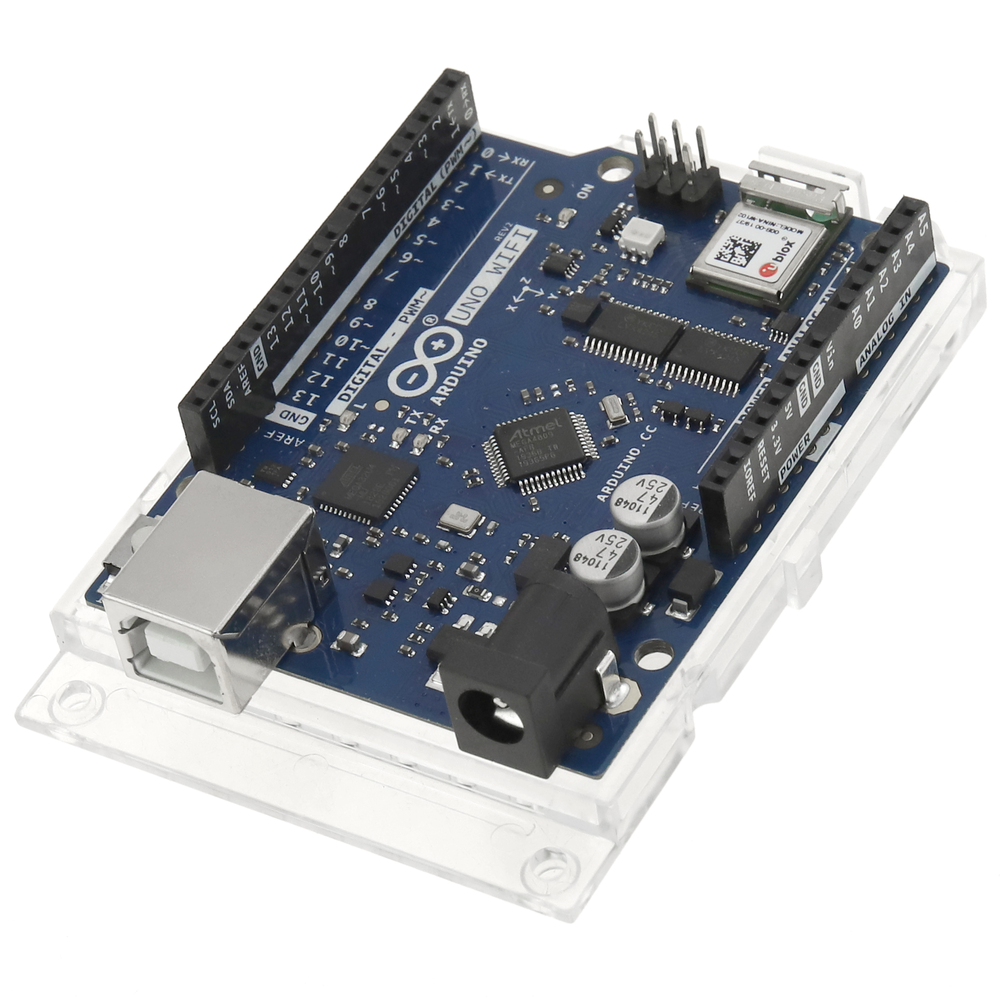
\includegraphics[width=0.25\textwidth]{resources/images/arduino.jpg}} & The arduino UNO Wifi Rev.2 is a very basic entry to IoT. It offers many different possibilities to build and expand it's functions. 
     \newline
     The Ardunino UNO Wifi Rev.2 has 14 digital input/output pins and 6 analog inputs. With its secure ECC608 crypto chip accelerator it is possible to directly connect the Arduino UNO Wifi Rev.2 to a Wifi network of your choice. \\
\addlinespace
\hline
\addlinespace
\raisebox{\ht\strutbox-\height}{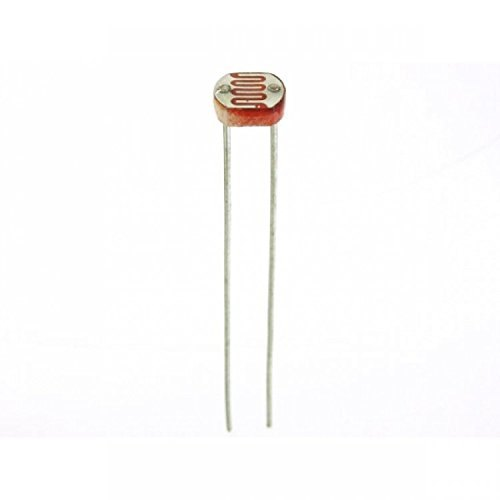
\includegraphics[width=0.25\textwidth]{resources/images/ldr.jpg}} & LDR's or Light Dependent Resistors are used in light/dark sensor circuits. The resistance of LDR normally is very high, sometimes as high as 1 Mega ohms, if they then get illuminated the resistance drops dramatically. \\
\addlinespace
\hline
\addlinespace
\raisebox{\ht\strutbox-\height}{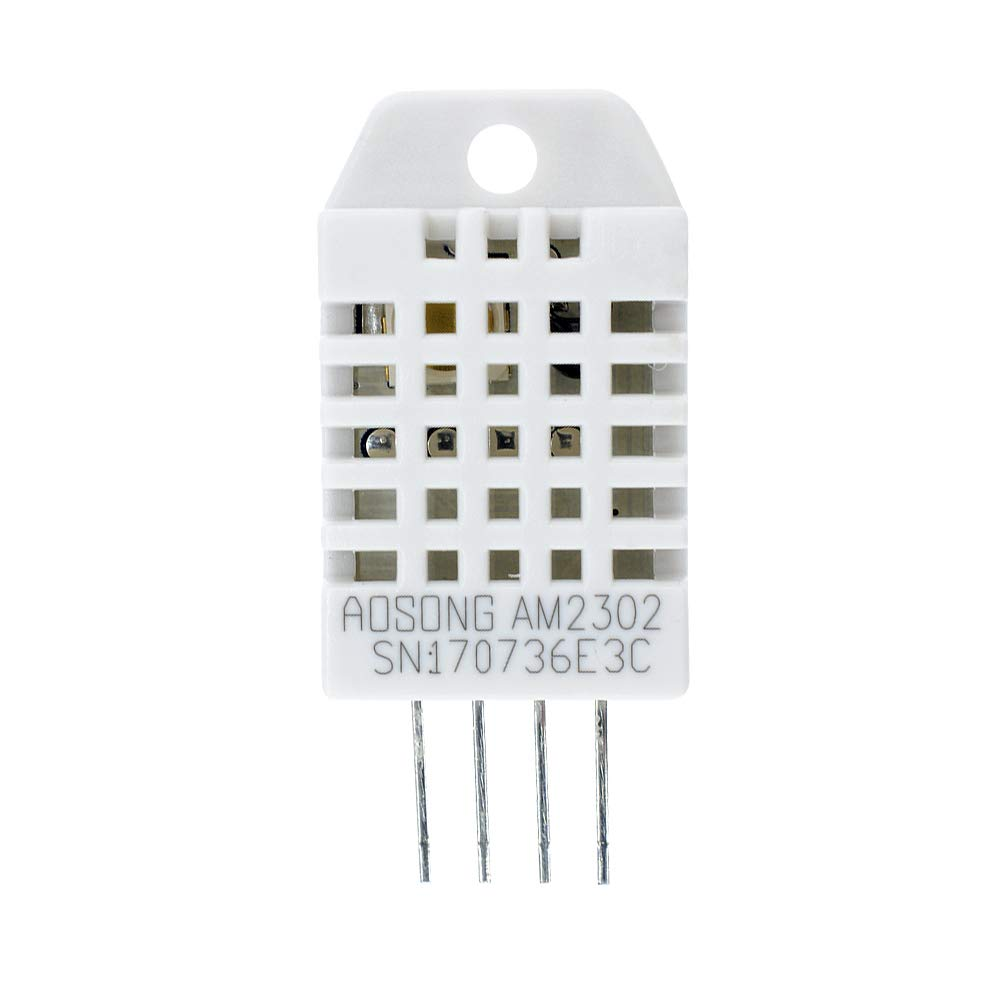
\includegraphics[width=0.25\textwidth]{resources/images/dt22.jpg}} & The DHT22 is low cost easy to use humidity and temperature sensor. It can measures humidity from 0-100\% with and accuracy of 2-5\% and the temperature from -40 to 80°C with accuracy +-0.5°C\\
\addlinespace
\hline
\addlinespace
\raisebox{\ht\strutbox-\height}{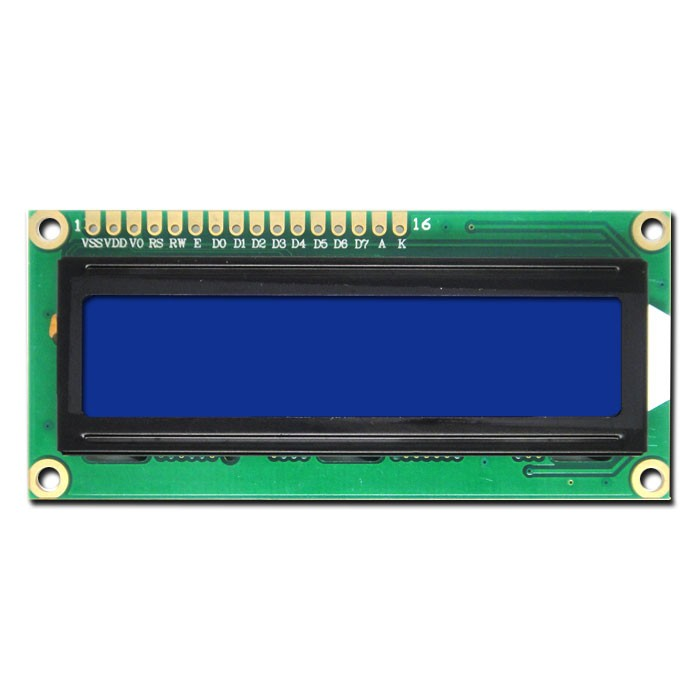
\includegraphics[width=0.25\textwidth]{resources/images/lcdDisplay.jpg}} &  The LCM1602C is a 2x16 LCD display which can be used to display information up to 32 characters over 2 lines.\\
\bottomrule
\end{tabularx}
    \newpage
    \subsection{Goal Definitions}
In this section, the goals of the bachelor thesis are defined, which are to be achieved, in addition, some optional goals are defined, which can be added as extensions if there is enough time. 
These are the "must" goals:
\begin{description}
\begin{itemize}
\item
The exchange of data should be largely anonymous. It should not be possible to know the data is being uploaded and who has read it. 
\item
The exchange of data must be protected and data must only be readable by authorized persons / hardware.  
\item
The data access should only be known to the authorized parties.  
\item
Document architecture and encryption.
\item
Implement the documented architecture and encryption in a prototype.
\item
Encryption and signing of the data using elliptic curves. If possible using elliptic curves, if not possible use AES / RSA.
\end{itemize}
\end{description}
\newline
These are the "optional" goals:
\begin{itemize}
\item
The security-relevant functions of Freenet should be used in the best possible way. 
\end{itemize}
    \newpage
    \chapter{Planing}
\section{Planing Methode}
For the planning of my bachelor thesis, I referred to the well-known project management method, the waterfall model. The waterfall model is a classic project management model that consists of successive phases. In contrast to agile project management models, each individual phase must be completed before the next one begins, since the individual phases build on each other. 
Although this project planning method has some disadvantages, the advantages outweigh them.
It allows you to better structure the work. Since phase after phase must be completed. It provides easy tracking, this because a waterfall model can be easily read and developed by all stakeholders without special certification or training.
The main disadvantage of the waterfall model is that it is difficult to make changes during the process. However, since the requirements and goals are already defined at the start of my bachelor thesis, the likelihood of changes during the process is negligible. 
\newline
On the next page you will find the waterfall model of my bachelor thesis. This was divided into 5 phases. Planning, Preparation, Documentation, Realization, Finalization.
Each of these phases has at least 1 milestone, which marks the end of the respective phase and at the same time the transition to the next phase.

    \newpage
    \section{Timeplan}
\begin{ganttchart}[Mile1/.style={milestone/.append style={fill=red}},
  Mile2/.style={milestone/.append style={fill=blue,shape=rectangle}}, x unit=0.4cm, y unit title=0.5cm, x unit chart=0.4cm, y unit chart=0.5cm]{1}{20}
  \gantttitle{2011}{20} \\
  \gantttitlelist{8,...,27}{1} \\
  \ganttgroup{Planing}{1}{3} \\
  \ganttgroup{Preparation}{4}{6} \\
  \ganttgroup{Documentation}{7}{10} \\
  \ganttgroup{Realization}{11}{17} \\
  \ganttgroup{Finalization}{18}{19} \\
  \ganttbar{Project filing}{1}{1} \\
  \ganttbar{Goal definiton}{2}{2} \\
  \ganttmilestone[Mile1]{Define exam date}{3}
  \ganttnewline
  \ganttbar{Encryption scheme analysis}{4}{5} \\
  \ganttmilestone[Mile1]{Define encryption scheme}{6}
  \ganttnewline
  \ganttbar{Document encryption scheme}{7}{7} \\
  \ganttbar{Create movie}{8}{8} \\
  \ganttbar{Create poster}{9}{9} \\
  \ganttmilestone[Mile1]{Book finished}{10}
  \ganttnewline
  \ganttmilestone[Mile1]{Finished movie}{10}
  \ganttnewline
  \ganttmilestone[Mile1]{Finished poster}{10}
  \ganttnewline
  \ganttbar{Lookup freenet security possibilities}{5}{7} \\
  \ganttbar{Implement freenet security}{8}{12} \\
  \ganttbar{Implement enc/dec prototype}{8}{13} \\
  \ganttbar{Finish prototype}{14}{15} \\
  \ganttbar{Test prototype}{16}{16} \\
  \ganttbar{Finish documentation}{12}{16} \\
  \ganttbar{Finish Presentation}{12}{16} \\
  \ganttmilestone[Mile1]{Public presentation}{17}
  \ganttnewline
  \ganttmilestone[Mile1]{Defense}{19}
  \ganttnewline
  \ganttlink{elem5}{elem6}
  \ganttlink{elem6}{elem7}
  \ganttlink{elem8}{elem9}
  \ganttlink{elem10}{elem11}
  \ganttlink{elem10}{elem12}
  \ganttlink{elem11}{elem15}
  \ganttlink{elem12}{elem14}
  \ganttlink{elem10}{elem13}
  \ganttlink{elem18}{elem23}
  \ganttlink{elem22}{elem23}
  \ganttlink{elem23}{elem24}
\end{ganttchart}
    \newpage
    \chapter{Architecture}
\section{Process architecture}
\begin{figure}[!htb]
    \centering
    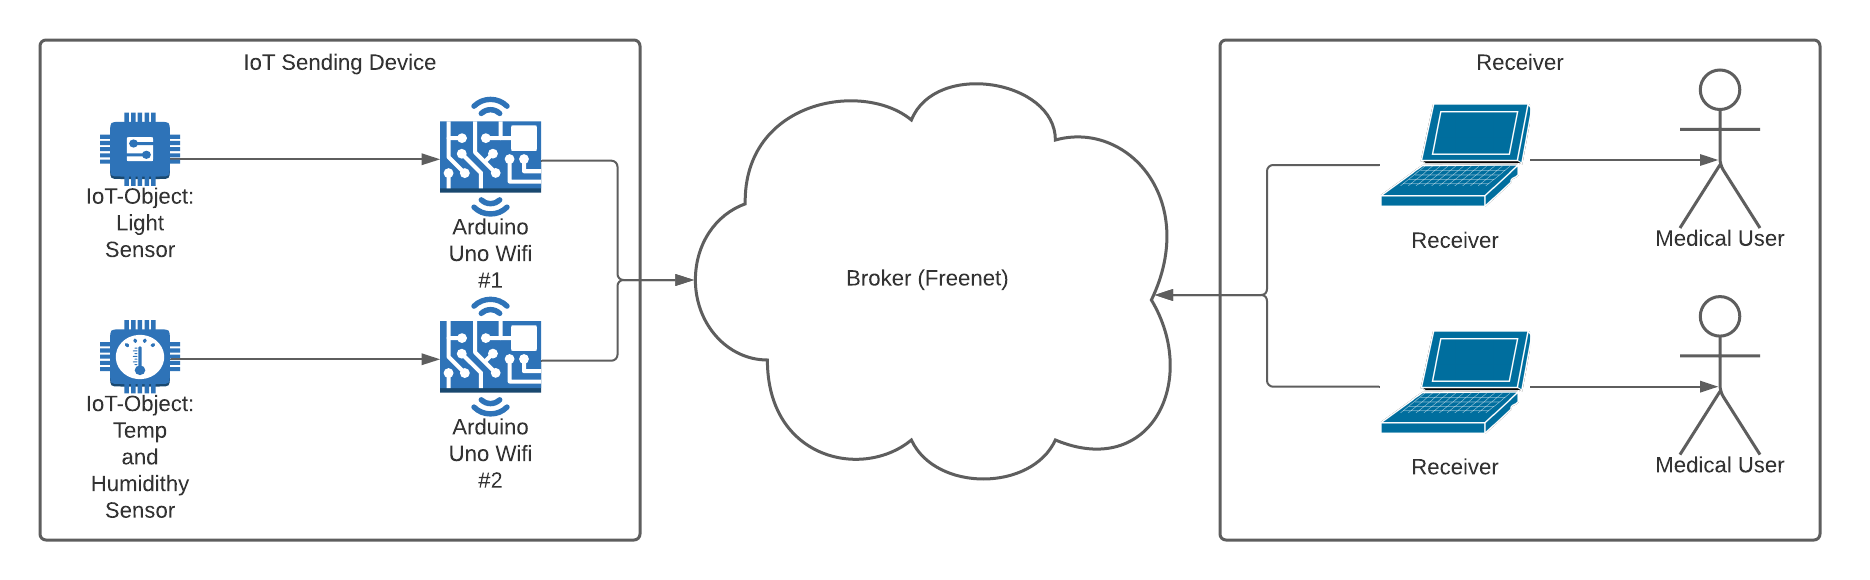
\includegraphics[width=15cm,height=19cm,keepaspectratio]{Architecture}
    \caption[Process overview]{Process overview}
    \label{fig:Architecture}
\end{figure}
\noindent
The figure above shows a complete process overview. Both endpoints are visible, on the left the IoT transmitter, the device that is with the patient and measures his vital signs. On the right is the endpoint device where the medical staff can evaluate the patient's values. The data exchange between the 2 endpoints takes place via a broker. In our architecture Freenet was used as broker. In order for the data to be transferred securely between the two endpoints, it must be protected from access and attack by third parties. This is done by an encryption between the two endpoints.
\newpage
\section{Arduino slot layout}
\begin{center}
\begin{figure}[!htb]
\subfigure{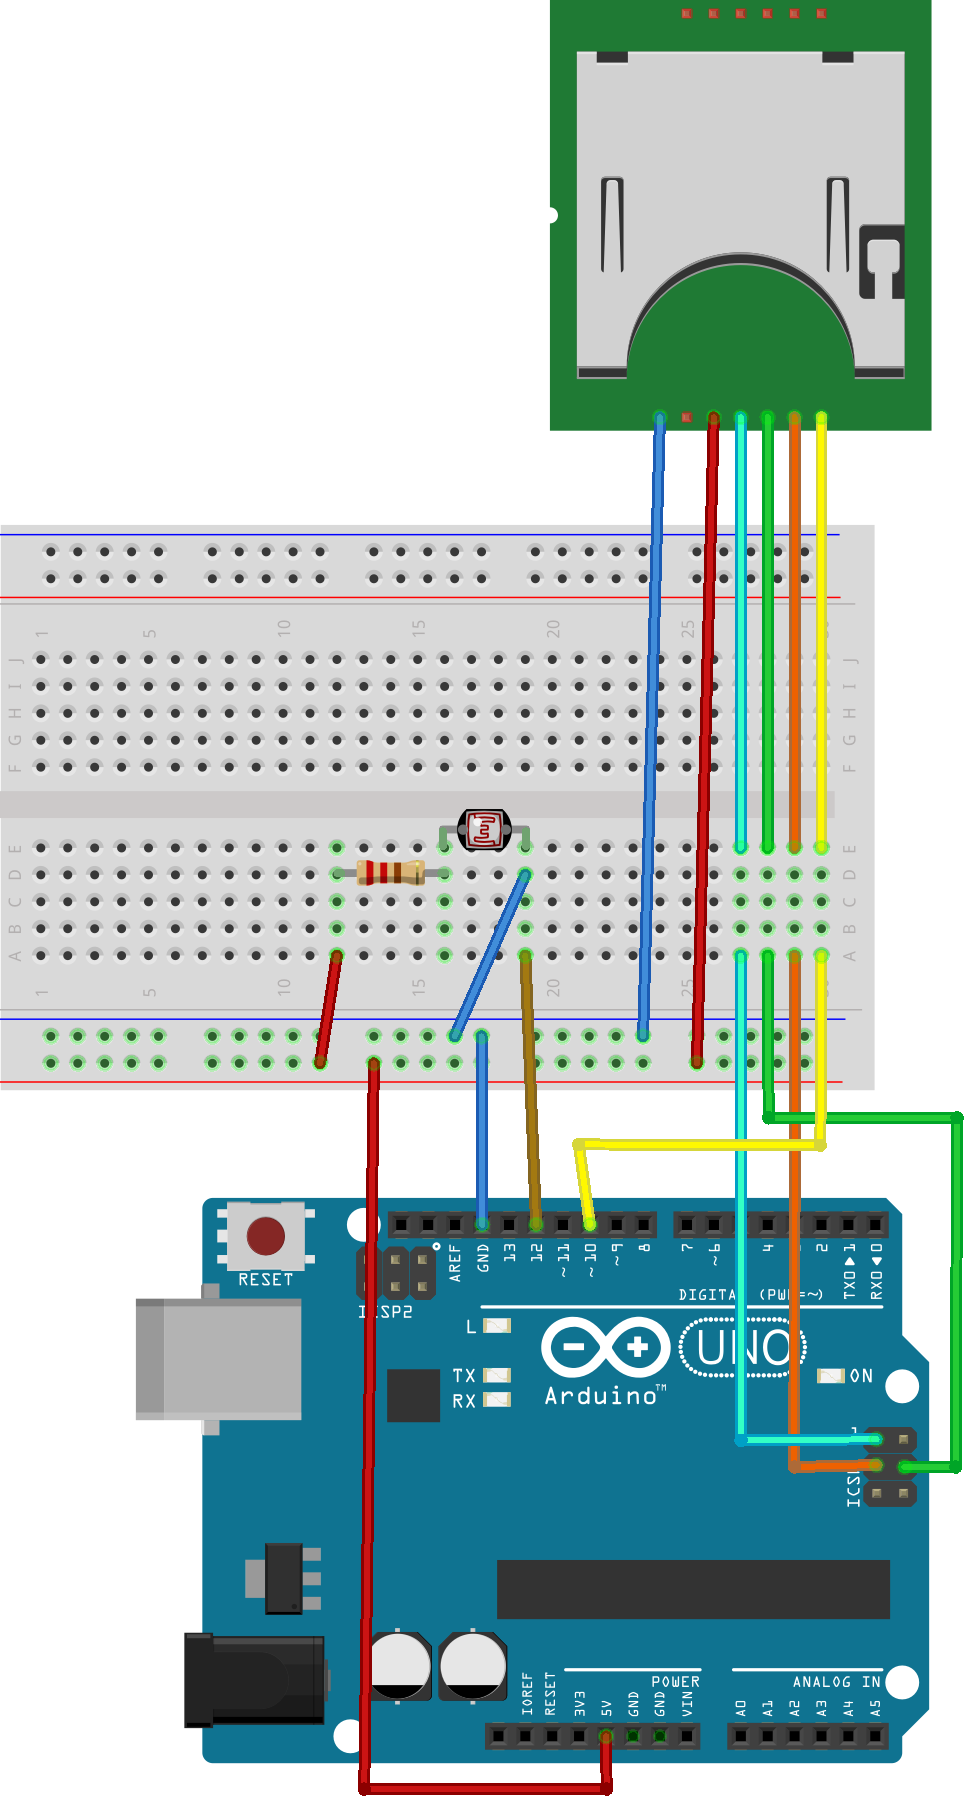
\includegraphics[width=6cm]{Arduino_LightSensor_Steckplatine}}
\hfill
\subfigure{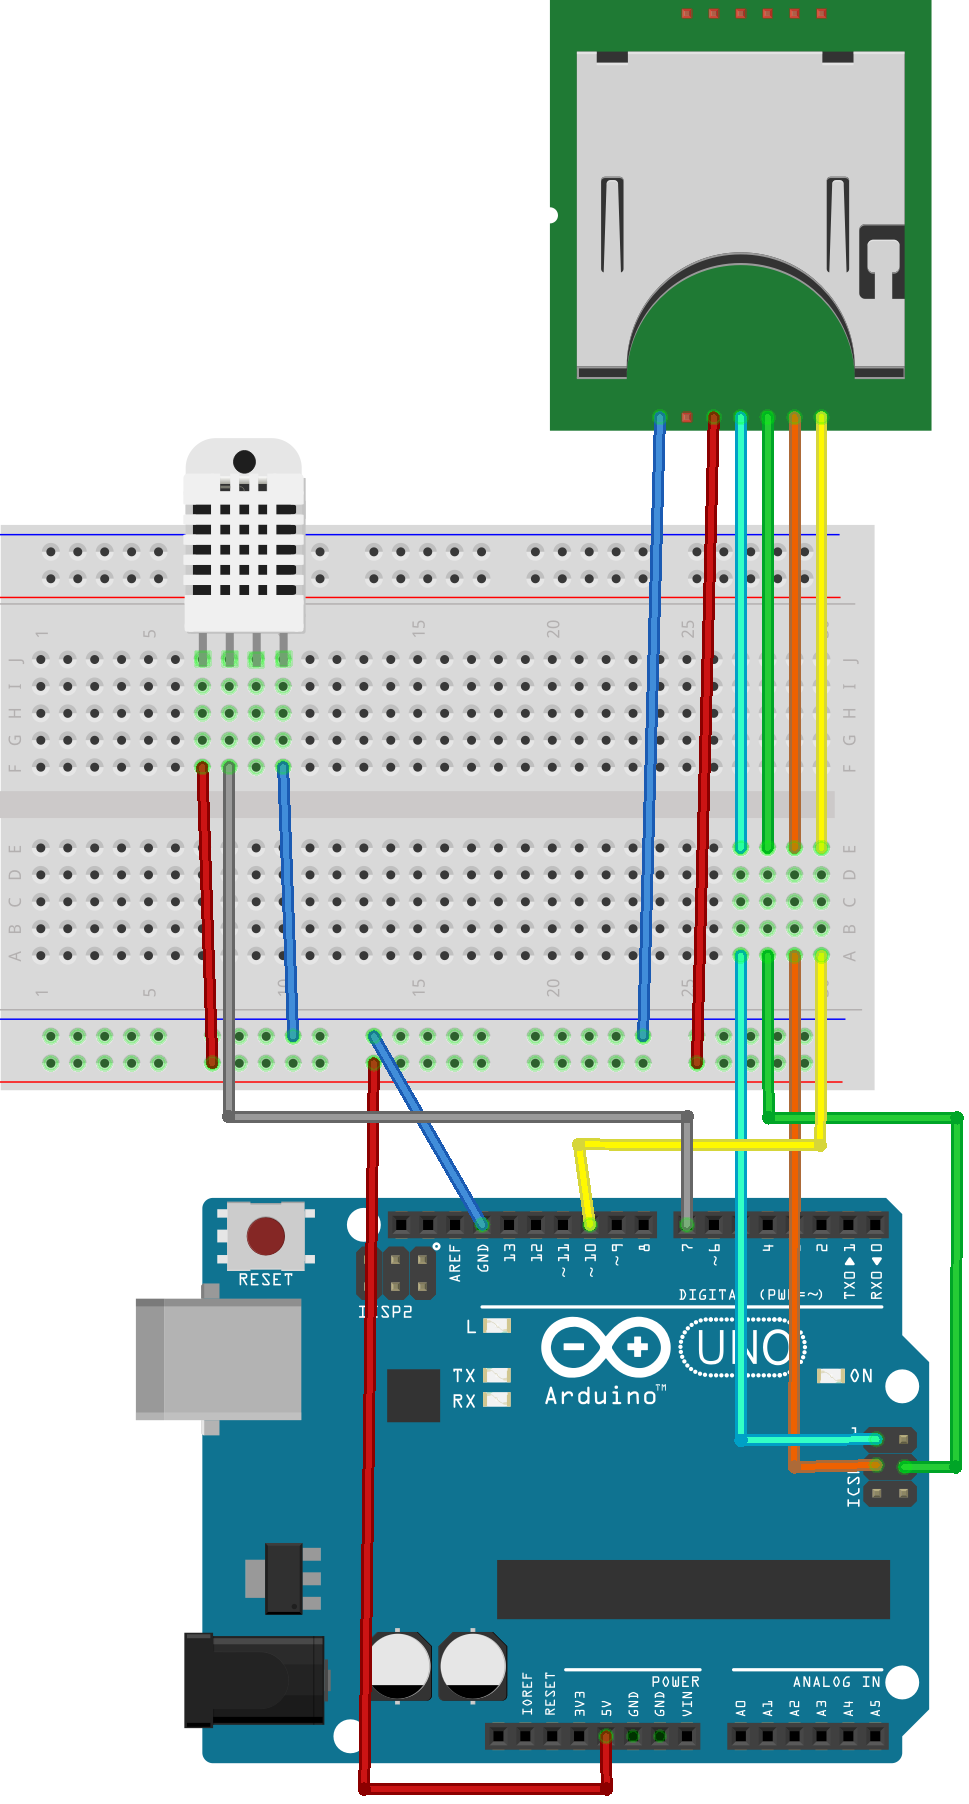
\includegraphics[width=6cm]{ArduinoTemp_Steckplatine}}
\caption{Arduino slot layouts}
\end{figure}
\end{center}
The two figures show an overview of the two Arduino cabling (IoT transmitter). The left figure shows the wiring with the light sensor and the right figure the wiring with the temperature sensor.
Bend Arduinos are also equipped with a micro SD card reader module, which is used to cache the communication data.
\newpage
\section{Preparations for initialization of communication}
In order for communication to occur between the two devices (sender and receiver), the two devices must exchange data over an insecure channel. Since the IoT devices are quite limited in terms of inputting data, they are equipped with a QR code. This QR code is scratchable, so that when the devices are received, it can be detected whether a QR code has already been read. The QR code contains a key that is used to send data to this device via Freenet. 
This initial data exchange takes place via an insecure channel. As soon as a recipient has registered with the sender via the QR code. A key exchange is executed via the insecure channel. In addition to the Key Exchange, new specific paths for the data exchange between the two devices are created and transmitted encrypted via the insecure channel. These new paths are then used for the subsequent data exchange.
\newpage
    \newpage
    \chapter{Mathematical basics}
\section{Diffie-Hellman key exchange}
\begin{center}
\begin{figure}[!htb]
    \centering
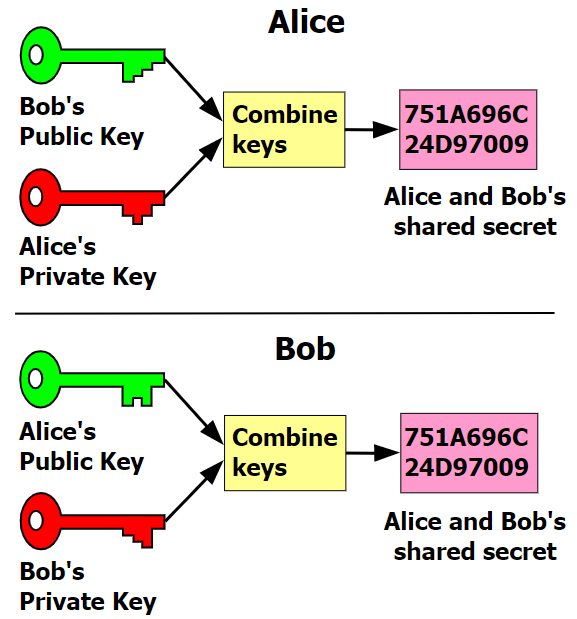
\includegraphics[width=6cm,height=8cm,keepaspectratio]{DHKeyExchange}
    \caption{Diffie Hellman key exchange}
    \label{fig:DHKeyExchange}
\end{figure}
\end{center}
\newline
The Diffie Hellman Key Exchange is a key agreement protocol. It allows two communication partners to agree on a common secret key via a public non-secure channel. This agreed secret key can then be used for a symmetric cryptosystem.
There are now different variants of the Diffie Hellman Key Exchange procedure, which are also used in various corners of the Internet.\cite{Diffie-Hellman_key_exchange}
\subsection{Mathematical basics}
In the following chapters, the mathematical basics of the asymmetric crypto methods based on the discrete logarithm are explained. The Diffie Hellman Key Exchange is composed of various mathematical aspects. The essential aspects that are necessary for the design and security analysis of the Diffie Hellman Key Exchange are explained in more detail in the following chapters.
\subsubsection{One-way function}
A Diffie Hellman Key Exchange uses certain mathematical basics, one of these basics is the one-way function(s). 
A one-way function is a mathematical function that is "easy" to calculate in terms of complexity theory, but very "difficult" to reverse. 
\begin{displaymath} \text{A mathematical one-way function }  f : X \to Y  \text{ must satisfy the following properties:}\end{displaymath}
    \begin{displaymath}
    \text{The calculation of }  y = f(x)  \text{ is "easy".}
    \end{displaymath}
This means that an algorithm exists that can calculate the value in polynomial time.
\newline
\begin{displaymath}
\text{The calculation of } f^-1(y) = x \text{is "hard".}
\end{displaymath}
This means that there is no "fast" algorithm for this problem that could solve it in polynomial time.\cite{Robshaw2011}
\subsubsection{Discrete exponential function and discrete logarithm}
The discrete exponential function \(b^x\mod m\) return the remainder when dividing \(b^x\) by m. 
And the inverse of the discrete exponential function is called discrete logarithm.
\newline
The big advantage of discrete exponential functions is that they can be calculated efficiently even with large exponents. So even functions with a number of more than hundred bits can be calculated within a second on the PC if implemented cleverly. For this to happen efficiently, both Euler's theorem
\newline 
(For all \(a, n \in \mathbb{N}\) with \(ggT(a,n) = 1\)
applies \(a^\varphi^(^n^) \equiv 1 (\mod n)\))
\newline 
as well as the Square & Multiply method are used.
\newline
But for the inverse, i.e. the discrete logarithm \(f(x) = b^x\modm\), no efficient and fast algorithm is known yet. Even with the greatest hardware effort and the best known algorithms, one only achieves calculation times that exceed the lifetime of our universe. Therefore, it can be assumed that the discrete exponential function is a one-way function according to today's knowledge. \cite{Diffie-Hellman_key_exchange}
\newpage
\subsubsection{Group theory}
Group theory deals with the algebraic structures of groups in mathematical space. 
Accordingly, a group consists of a set of things (numbers, symbols, objects, motions) and a calculus (a linkage \(*\)) that specifies how to deal with the set. This calculation rule is bound to certain rules, the so-called group axioms:
\begin{itemize}
    \item The combination of two elements of the set results in an element of the same set. (Completeness of the set)
    \item For the combination of the elements the bracketing is not of importance, i.e., it is valid \((a * b) * c = a * (b * c)\) for all \(a,b,c\). (associative law)
    \item There is an element \(\varepsilon\) in the set, which does nothing with respect to the conjunction, i.e. a \(*\)-neutral element:\(a * \varepsilon = \varepsilon * a = a\) for all \(a\)
    \item For each element \(a\) there is a reverse element with respect to the link, i.e. an \(*\text{-inverse}\) element \(a^*\). This element has the property of yielding the neutral element when it is linked with \(a\): \(a^* * a = a * a^* = \varepsilon\).
\end{itemize}
A group is therefore defined as follows: It is a pair \((G, *)\). Here \(G\) is a set and \(*\) is the linkage to \(G\). 
The following figure can be described accordingly:  \cite{Diffie-Hellman_key_exchange}
\begin{eqnarray*}
*: G \times G \to G (a, b) \mapsto a * b
\end{eqnarray*}
\subsubsection{Prime residual class group}
In arithmetic, the integers relatively prime to n from the set \(\{0,1,....,n-1\}\) of \(n\) non-negative integers form a group under multiplication of modulo \(n\).
This group is called the multiplicative group of integers modulo \(n\).
\newline
This type of group plays a significant role in cryptography because they are finite abelian groups with respect to multiplication.
An important property of the prime residue class is that for every prime residue class \(a + n\mathbb{Z}\) there exists a prime residue class \(b + n\mathbb{Z}\) such that holds:
\begin{eqnarray*}
ab \equiv 1 \pmod n
\end{eqnarray*}
The prime residue class \(b + n\mathbb{Z}\) is therefore the inverse element of \(a + n\mathbb{Z}\) with respect to the multiplication in the prime residue class group \(\mathbb{Z}^*_n\).\cite{Multiplicative_group_of_integers_modulo_n}
\newpage
\subsubsection{Primitive root modulo n}
Certain elements of prime residue class groups are called primitive roots in scale theory. The primitive root has a primitive property, through this property it is possible to represent each element of the primitive residue class group by means of one of its powers.
For example, the number 3 is a primitive root modulo 7, since holds:\cite{Primitive_root_modulo_n}
\begin{eqnarray*}
3^1\equiv3  \pmod 7 \\
3^2\equiv2  \pmod 7 \\
3^3\equiv6  \pmod 7 \\
3^4\equiv4  \pmod 7 \\
3^5\equiv5  \pmod 7 \\
3^6\equiv1  \pmod 7 \\
\end{eqnarray*}
\section{Elliptic Curves}
Elliptic curves are special algebraic curves on which addition is geometrically defined. They play an important role in cryptography to construct secure encryption methods. This due to the various properties of elliptic curves. For example, the discrete logarithm problem is much harder to compute on an elliptic curve than on finite solids.  
For the representation of elliptic curves, so-called affine planes with a point at infinity are used. 
However, elliptic curves can also be defined in arbitrary bodies, but only elliptic curves over finite bodies are used in cryptography.
\newline
\newline
An elliptic curve is defined as follows according to Willems.
\newline
Let \(\mathbb{K}\) be a body of characteristic not equal to 2 and 3. 
\newline
A polynomial equation of the form \(\text{E: }y^2 = x^3 + ax + b\) with \(a, b \in \mathbb{K}\) with discriminant \(\Delta = 4a^3 + 27b^2 \neq 0\) is called an elliptic curve.
\newline
The condition \(\Delta \neq 0\) ensures that the polynomial \(x^3 + ax + b\) has three pairwise different zeros.\cite{ellipticCurves}
\newpage
\subsection{Elliptic Curve Diffie-Hellman (ECDH)}
The elliptic curve Diffie Hellman (ECDH) differs from the general Diffie Hellman in that it is based on the discrete logarithm problem of the elliptic curve (ECDLP) as opposed to the discrete logarithm problem (DLP) of the general Diffie Hellmann. The Elliptic Key Diffie Hellmann is an anonymous key agreement protocol that allows 2 parties to share a secret over a insecure channel. Each party has a public-private key pair, of which only the public key is used for the exchange. The private key remains with the party and is needed to create the shared secret.
\newline
The ECDH works as follows. A and B agree on the elliptic curve group \(\mathbb{E}\) of order \(n\) and \(a\) primitive element \(\mathbb{P}\) in \(\mathbb{E}\), which then also has the order \(n\). \(\mathbb{E} \text{, } n \text{ and } \mathbb{P}\) are assumed to be known to the adversary. The ECDLP, which the ECDH is based on, is defined as the computation of the integer \(k\) given \(\mathbb{P} \text{ and } \mathbb{Q}\) such that \(\mathbb{Q} = [k]\mathbb{P}\). The ECDH
let A and B compute a shared secret key S, using the property of the ECDLP as described below. A selects an integer \(a\) in the range [2, n-1], computes
\(\mathbb{Q} = [a]\mathbb{P}\) and sends \(\mathbb{Q}\) to B. B on the other hand selects an integer \(b\) in the range [2, n-1], computes \(\mathbb{R} = [b]\mathbb{P}\) and sends \(\mathbb{R}\) to A. A and B receives \(\mathbb{R} \text{ and } \mathbb{Q}\) respectively, and computes the shared secret key 
S; \(S = [a]\mathbb{R} = [b]\mathbb{Q} = [a][b]\mathbb{P} = [a ∗ b \mod{n})]\mathbb{P}\). Both A and B get the same value for S, and the shared key is established.\cite{ECDH}
\newline
\begin{center}
\begin{figure}[!htb]
    \centering
    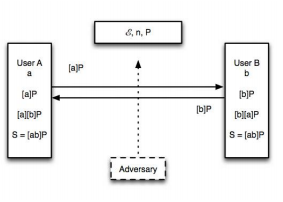
\includegraphics[width=9cm,height=11cm,keepaspectratio]{ecdh}
    \caption{Elliptic curve Diffie Hellman}
    \label{fig:ecdh}
\end{figure}
\end{center}
\newpage
    \newpage
    \chapter{Processes and protocols}
\section{Initialization of communication}
In order to establish a connection between the transmitter and receiver, these two devices must register with each other. Since the IoT transmitter is a device with very limited functions, it cannot register the receiver by input. Each transmitter is therefore equipped with a QR code. This QR code contains the address that can be used to communicate with the transmitter via Freenet.
The receiver registers the transmitter via its QR code. The address of the recipient is then transmitted to the sender via Freenet. The sender registers the recipient's address.
As soon as both sides have registered each other's communication path, an EC is sent to the receiver.
an ECDH (Elliptic Curve Diffie Hellman) is performed by both sides using the SecP256 elliptic curve. 
For this, an ECC (elliptic curve cryptography) key pair is created by both sides. 
The public key of the key pair is then forwarded to the other side via Freenet. Both sides calculate a shared secret after receiving the public key from the other side. Up to this point, the entire communication takes place on a non-secure channel. 
As soon as both parties have calculated the shared secret, both sides create new connection paths on Freenet. These paths are then encrypted with the shared secret and transferred to the other side.
Further communication then takes place via the secure channel created in this way.
\newpage
\subsection{SecP256r1 Elliptic curve}
SECP256r1 is an elliptic curve defined in SEC 2. It is an elliptic curve in the field \(z_p\), where \(p\) is a 256-bit prime. The "r" stands for random. The elliptic curve SECP256r1 has another sibling curve, the SECP256k1. The "k" stands for Koblitz. A Koblitz curve has some special properties that allow it to implement the group operations more efficiently. However, one assumes that a small security trade-off takes place, since often a greater "randomness" of the selected parameters leads to a higher security. For this reason, the elliptic curve SECP256r1 was used for the implementation of the prototype.
\begin{center}
\begin{figure}[!htb]
    \centering
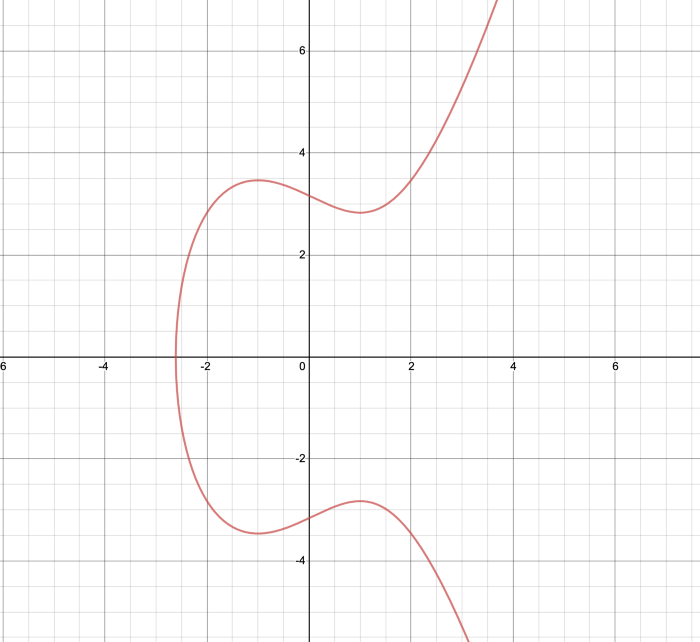
\includegraphics[width=6cm,height=8cm,keepaspectratio]{resources/images/NISTP256Curve.png}
    \caption{SecP256k1 Elliptic curve}
    \label{fig:DHKeyExchange}
\end{figure}
\end{center}
\newpage
\section{Initialization scheme}
\begin{center}
\rotatebox{90}{
\scalebox{0.7}{
\tcbox[top=0pt,left=0pt,right=0pt,bottom=0pt]{
\pseudocodeblock{
 \textbf{IoT sender} \< \< \textbf{Broker} \< \< \textbf{IoT receiver} \\[][\hline]
  \< \< \< \< \text{Register sender Freenet path } \\
  \< \< \< \sendmessageleft{top=Upload receiver Freenet path} \< \\
  \< \< \text{store receiver path} \< \< \\
  \< \sendmessageright{top=Get receiver path} \< \< \< \\
  \< \sendmessageleft{top=return receiver path} \< \< \< \\
  \text{Register receiver Freenet path} \< \< \< \< \\
\text{Gen random ECC key pair}  \< \< \< \< \text{Gen random ECC key pair} \\
 \< \sendmessageright{top=Upload sender pubkey} \< \< \sendmessageleft{top=upload receiver pubkey} \< \\
 \< \< \text{store information} \< \< \\
 \< \sendmessageleft{top=get receiver pubkey} \< \< \sendmessageright{top=get sender pubkey} \< \\
   \text{Calculate shared secret} \< \< \< \< \text{Calculate shared secret} \\
 \text{Gen new SSK Keypair} \< \< \< \< \text{Gen new SSK Keypair} \\
 \text{(Freenet path)} \< \< \< \< \text{(Freenet path)} \\
 \text{Encrypt Freenet path} \< \< \< \< \text{Encrypt Freenet path} \\
 \< \sendmessageright{top=Upload Freenet path} \< \< \sendmessageleft{top=Upload Freenet path} \< \\
 \< \< \text{store information} \< \< \\
 \< \sendmessageleft{top=get Freenet path} \< \< \sendmessageright{top=get Freenet path} \< \\
 \text{store receiver Freenet path} \< \< \< \< \text{store sender Freenet path} \\
}
}
}
}
\end{center}

    \newpage
    \section{Send and receive data}
Once the connection between a transmitter and a receiver is established, the two devices proceed to the next step. The IoT transmitter reads the required information from the SD card. It thus obtains the Freenet path of the receiver and the key for encrypting the data. 
It then reads the data from the sensor. Formats it and encrypts it. The data is then uploaded in encrypted form from the IoT transmitter to the receiver's Freenet path.
The receiver regularly checks whether new data has already been uploaded from the transmitter. If it detects that new data has been uploaded, it downloads it and verifies it. For this purpose, it decrypts the received data.  If the data has been downloaded correctly, the receiver sends the sender a confirmation that it has received the data via its Freenet path.
\newline
An IoT transmitter only sends the data if it has received confirmation of the previous upload of data, thus ensuring that the receiver is still active and therefore still receiving data.
\newpage
\section{Communication scheme}
\begin{center}
\rotatebox{90}{
\scalebox{0.7}{
\tcbox[top=0pt,left=0pt,right=0pt,bottom=0pt]{
\pseudocodeblock{
 \textbf{IoT sender} \< \< \textbf{Broker} \< \< \textbf{IoT receiver} \\[][\hline]
 \text{Get stored Freenet path} \< \< \< \< \\
 \text{Get shared secret} \< \< \< \< \\
 \text{Encrypt information} \< \< \< \< \\
 \< \sendmessageright{top=Upload info} \< \< \< \\
 \< \<  \text{store info} \< \< \\
 \< \sendmessageleft{top=Upload result} \< \< \< \\
 \< \< \< \sendmessageright{top=Get info} \< \\ 
 \< \< \< \< \text{Get shared secret} \\
 \< \< \< \< \text{Decrypt information} \\
  \< \< \< \< \text{Get stored Freenet path} \\
 \< \< \< \< \text{Encrypt receive confirmation} \\
 \< \< \< \sendmessageleft{top=Send receive confirmation} \< \\
 \< \<  \text{store receive confirmation} \< \< \\
 \< \sendmessageleft{top=get receive confirmation} \< \< \< \\
 \text{Get shared secret} \< \< \< \< \\
 \text{start over} \< \< \< \< \\
}
}
}
}
\end{center}
    \newpage
    \chapter{Freenet}
\section{FCPv2 protocol}
Freenet uses a simple, text-based protocol called FCPv2 (Freenet Client Protocol) to allow third-party applications to interact with Freenet. \newline
Functionalities supported by the FCPv2 Protocol are:\cite{FCP}
\begin{itemize}
    \item Inserting of data into Freenet
    \item Retrieval of data from Freenet
    \item Querying the status of Freenet
    \item Managing the other Freenet nodes that are connected to your own node.
\end{itemize}
\newpage
\subsection{ClientHello}
The first message sent from the third-party client to the node on a given connection is always the ClientHello message. No other messages are allowed to be sent to the node before the ClientHello is sent. The node will always respond with a NodeHello message.
\begin{verbatim}
    ClientHello
    Name=My Freenet Client
    ExpectedVersion=2.0
    EndMessage
\end{verbatim}
\begin{tabularx}{\textwidth}{p{3cm}|p{2cm}|p{2.5cm}|p{5.5cm}}
\toprule
    Field & Possible values & Mandatory? & Description \\
\midrule 
Name & Arbitrary string, on one line & yes & A name to uniquely identify the client to the node. \\
\addlinespace
\hline
\addlinespace
ExpectedVersion & 2.0 & yes & The version of FCP to expect. In this case it will always be 2.0 \\
\bottomrule
\end{tabularx}
\newpage
\subsection{NodeHello}
The NodeHello message is the reply a node sends after receiving a ClientHello message from a client.
\begin{verbatim}
    NodeHello
    CompressionCodecs=4 - GZIP(0), BZIP2(1), LZMA(2), LZMA_NEW(3)
    Revision=build01475
    Testnet=false
    Version=Fred,0.7,1.0,1475
    Build=1475
    ConnectionIdentifier=6f467be43d838f8e02877e7f176a73bd
    Node=Fred
    ExtBuild=29
    FCPVersion=2.0
    NodeLanguage=ENGLISH
    ExtRevision=v29
    EndMessage
\end{verbatim}
\begin{tabularx}{\textwidth}{p{3cm}|p{3cm}|p{7.5cm}}
\toprule
    Field & Example or [range] & Description \\
\midrule 
FCPVersion & 2.0 &  The version of FCP being utilized for this connection. \\
\addlinespace
\hline
\addlinespace
Node & Fred & \\
\addlinespace
\hline
\addlinespace
Version & Fred, 0.7, 1.0, 1475 & A comma-delimited list consisting of 
\begin{itemize}
    \item node name
    \item node version
    \item protocol version
    \item build number
\end{itemize}\\
\addlinespace
\hline
\addlinespace
Build & 1475 & \\
\addlinespace
\hline
\addlinespace
Revision & build01475 & \\
\addlinespace
\hline
\addlinespace
ExtBuild & 29 & The build of freenet-ext.jar being utilized by the node.\\
\addlinespace
\hline
\addlinespace
ExtRevision & v29 & The revision of freenet-ext.jar being utilized by the node.\\
\addlinespace
\hline
\addlinespace
Testnet & true, false & \\
\addlinespace
\hline
\addlinespace
Compression Codecs & 4 - GZIP(0), BZIP2(1), LZMA(2), LZMA_NEW(3) & A list of the compression codecs supported by the node.\\
\addlinespace
\hline
\addlinespace
Connection Identifier & 6f467be43d838f8 e02877e7f176a 73bd & A unique connection identifier, reported in hexadecimal format.\\
\addlinespace
\hline
\addlinespace
NodeLanguage & ENGLISH & The language currently utilized by the node.\\
\bottomrule
\end{tabularx}
\subsection{ClientPut}
The ClientPut message is used to specify an insert into Freenet of a single file. This file can be inserted by referring to a file on the disk, including the data directly in the message or redirecting to another key.
\begin{verbatim}
    ClientPut
    URI=KSK@
    Metadata.ContentType=text/plain
    Identifier=My Test Insert
    DataLength=4
    Data
    <Data>
\end{verbatim}
\begin{tabularx}{\textwidth}{p{3cm}|p{2cm}|p{2.5cm}|p{5.5cm}}
\toprule
    Field & Possible values & Mandatory? & Description \\
\midrule 
URI & CHK@ KSK@ SSK@ USK@ & yes & The type of key to insert. \\
\addlinespace
\hline
\addlinespace
Metadata. ContentType & Any MIME type & no & The MIME type of the data being inserted. \\
\addlinespace
\hline
\addlinespace
Identifier & Arbitrary text string & yes & This is just for client to be able to identify files that have been inserted. \\
\addlinespace
\hline
\addlinespace
DataLength & Integer from 0 to ? & yes & The length of the data file being included in this FCP message. \\
\addlinespace
\hline
\addlinespace
Data &  &  & Indicates the end of the message. The data follows this line. \\
\bottomrule
\end{tabularx}
\newpage
\subsection{ClientGet}
The ClientGet message is used to specify a get of a single file from Freenet.
\begin{verbatim}
    ClientGet
    URI=KSK@
    Identifier=My Test Identifier
    EndMessage
\end{verbatim}
\begin{tabularx}{\textwidth}{p{3cm}|p{2cm}|p{2.5cm}|p{5.5cm}}
\toprule
    Field & Possible values & Mandatory? & Description \\
\midrule 
URI & CHK@ KSK@ SSK@ USK@ & yes & The type of key to insert. \\
\addlinespace
\hline
\addlinespace
Identifier & Arbitrary text string & yes & This is just for client to be able to identify files that have been inserted. \\
\bottomrule
\end{tabularx}
\newpage
\subsection{DataFound}
DataFound indicates a successful fetch of the key, but does not actually include the data.
\begin{verbatim}
    DataFound
    Identifier=Request Number One
    Metadata.ContentType=text/plain;charset=utf-8
    DataLength=37261
    EndMessage
\end{verbatim}
\begin{tabularx}{\textwidth}{p{3cm}|p{3cm}|p{7.5cm}}
\toprule
    Field & Example or [range] & Description \\
\midrule 
Identifier & Arbitrary text string & This is just for client to be able to identify files that have been inserted. \\
\addlinespace
\hline
\addlinespace
Metadata. ContentType & Any MIME type & The MIME type of the data being inserted. \\
\addlinespace
\hline
\addlinespace
DataLength & Integer from 0 to ? & The length of the data file being included in this FCP message. \\
\bottomrule
\end{tabularx}
\newpage
\subsection{AllData}
AllData is a message from the node returning data from the node.
\begin{verbatim}
    AllData
    Identifier=Request Number One
    DataLength=37261 // length of data
    StartupTime=1189683889
    CompletionTime=1189683889
    Metadata.ContentType=text/plain;charset=utf-8
    Data
     <37261 bytes of data>
\end{verbatim}
\begin{tabularx}{\textwidth}{p{3cm}|p{3cm}|p{7.5cm}}
\toprule
    Field & Example or [range] & Description \\
\midrule 
Identifier & Arbitrary text string & This is just for client to be able to identify files that have been inserted. \\
\addlinespace
\hline
\addlinespace
DataLength & Integer from 0 to ? & The length of the data file being included in this FCP message. \\
\addlinespace
\hline
\addlinespace
StartupTime & Time & The startup time of the GetRequest. \\
\addlinespace
\hline
\addlinespace
CompletionTime & Time & The completion time of the GetRequest. \\
\addlinespace
\hline
\addlinespace
Metadata. ContentType & Any MIME type & The MIME type of the data being inserted. \\
\bottomrule
\end{tabularx}
\newpage
\subsection{GenerateSSK}
The GenerateSSK message is used to ask the node to generate us an SSK keypair. Response will come back in a SSKKeypair message.
\begin{verbatim}
    GenerateSSK
    Identifier=My Identifier Blah Blah
    EndMessage
\end{verbatim}
\begin{tabularx}{\textwidth}{p{3cm}|p{2cm}|p{2.5cm}|p{5.5cm}}
\toprule
    Field & Possible values & Mandatory? & Description \\
\midrule 
Identifier & Arbitrary text string & yes & This is just for client to be able to identify files that have been inserted. \\
\bottomrule
\end{tabularx}
\newpage
\subsection{SSKKeypair}
Is a message sent from the Freenet node to a client program in response to the client issuing a GenerateSSK command.
\begin{verbatim}
    SSKKeypair
    InsertURI=freenet:SSK@AKTTKG6YwjrHzWo67laRcoPqibyiTdyYufjVg54fBlWr,
               AwUSJG5ZS-FDZTqnt6skTzhxQe08T-fbKXj8aEHZsXM/
    RequestURI=freenet:SSK@BnHXXv3Fa43w~~iz1tNUd~cj4OpUuDjVouOWZ5XlpX0,
               AwUSJG5ZS-FDZTqnt6skTzhxQe08T-fbKXj8aEHZsXM,AQABAAE/
    Identifier=My Identifier from GenerateSSK
    EndMessage
\end{verbatim}
\begin{tabularx}{\textwidth}{p{3cm}|p{3cm}|p{7.5cm}}
\toprule
    Field & Example or [range] & Description \\
\midrule 
InsertURI & inserting URI & Consists the URI needed to insert to freenet. \\
\addlinespace
\hline
\addlinespace
RequestURI & request URI & Consists the URI needed to request from freenet. \\
\addlinespace
\hline
\addlinespace
Identifier & Arbitrary text string & This is for the Client to Identify to witch GenerateSSK Request this Keypair is. \\
\bottomrule
\end{tabularx}
\newpage
    \newpage
    \chapter{Attacks an Prevention}
The following chapter describes various possible attack scenarios and the possible solutions to prevent them. 
The following attacks are considered: 
\begin{itemize}
    \item{Spoffing of the data:}
    \SubItem{The information stored on the broker can be manipulated by anyone who can connect to the Freenet Node and also has knowledge of the Freenet URIs. 
To prevent this from happening, Freenet URIs must be exchanged in encrypted form for each new connection. }
    \item{Interruption of the data flow by flooding Freenet:}
        \SubItem{Freenet runs as a node on a device, the exact behavior of Freenet and the effects due to the high load need to be further investigated. (Packet loss and availability)  }
    \item{Physical attack:}
        \SubItem{There are several possible physical points of attack, one of which is the IoT transmitter. In our prototype, it is equipped with an SD card. Stored on it are all the information about the connections to the receivers. This data is stored on the SD card in encrypted form. However, the key for this encryption is stored on the EEPROM of the IoT transmitter. Furthermore, we have a Freenet node that is also physically located on site. If this is accessed, or if the permissions are not set correctly, a lot of information can be tapped here as well.}
    \newpage
    \item{Man in the Middle:}
        \SubItem{The man in the middle attack is very heavy here due to the use of Freenet. Since here is the only point of attack for a Man in the Middle. There is, however, the possibility that an attacker could pretend to be the recipient of the sender's QR code and thus establish his own communication with the sender. To ensure that the QR code has not yet been read out for registration before it is used at the customer's premises, it is delivered as a scratch-off zone on a piece of paper. If the QR code has already been scratched off, it can be assumed that it has already been read out.}
    \item{Shell injection:}
        \SubItem{When creating the receiver software, the first attempt was made to use the same ECC library as for the transmitter. Since this is a C library, it was provided as a .dll. However, since the use of this DLL leads to a high risk of a shell incjection, it was decided to use a specific C\# library that performs the calculations of the elliptic curve and thus has a much lower risk of a shell injection.}
\end{itemize}
    \newpage
    \chapter{Problems}
During the work on my bachelor thesis I stumbled more and more over single major as well as minor problems. 
These are both in the creation of the prototype as well as in planning and the effort of the work in addition to the daily work.
However, more problems have arisen during the creation of the prototype. Thus I had to determine with the wiring after several unsuccessful attempts, which the slots of the Arduino UNO Wifi Rev3 are not identical with the normal Arduino Uno. 
\newline
So that the cabling of the so-called ICSP ports that enable the control of the Micro SD Card Reader module via the instructions described in the Arduino Uno on the digital ports of 7-13 are present, so they are not connected to the digital ports on the Arduino Uno Wifi Rev3. In order to find out where to find these ports, I spent several hours studying the schematic of the chipset. Once I understood the schematic, I was able to connect the SD card module without any problems.
\newline
One problem that was identified during the development of the prototype is the roundtrip time. Since it is very important in medicine to always get the most current data in order to always know directly about the condition of the patient. Because of the using of a broker it came to the fact that we had an increased roundtrip time. We have now decided on a maximum roundtrip time of 10s for the prototype. Since this would probably be too much for a productive implementation, we would have to take care of this problem again.
Another problem was the ECDH (Elliptic Curve Diffie-Hellmann) key exchange. Since I only found a C library for the Arduino, I had to use another library for the receiver, which is a C# application. 
The use of these 2 different libraries leads however at first also to problems, since the Shared Secret computed at the end did not agree.
Furthermore, the library for using the FCP protocol for "C" was outdated and no longer current, so I decided to combine the required messages in a separate small "library".
    \newpage
    \chapter{Conclusion}
The goal of this work was to analyze and develop a prototype that makes it possible to detach the communication of IoT data from the manufacturer of the devices. So that they no longer have to struggle with the problem of dependence on the manufacturer. 
Based on this problem, a new communication path for the IoT data had to be developed. The goal was to exchange the data as anonymously and securely as possible. 
In addition, unauthorized parties should be prevented from gaining access to the data or its information.
In order to implement these goals, communication via Freenet was targeted. Freenet itself already stands for an anonymized decentralized network with which data can be exchanged. 
However, since anyone who connects to my Freenet node can see this data, the data had to be additionally protected.
For this an Elliptic Curve Diffie-Hellmann Key Exchange was executed. With this it was possible to transfer the data additionally in encrypted form.
Even if with the work defined in this thesis and its prototypes it was shown that a communication of IoT data can be executed secured and anonymous over Freenet. Nevertheless, some further work is available. 
The communication over Freenet is currently not very performant, here would be one of the biggest approaches for improvement. Additionally, the current prototype only supports communication between 2 parties at a time. Therefore, it is also possible to start here to enable multiparty usage. 
These are only two of a few approaches that could lead to an improvement of the prototypes.
During the implementation of this work, I was able to implement much of what I learned in theory in a practice-oriented prototype. In addition, my theoretical knowledge helped me a lot in creating the architecture of the new communication path. All in all, I was able to put a lot of what I had learned into practice in this prototype.
    \newpage
    \nocite{*}
\printbibliography[heading=bibintoc]
    \newpage
    \cleardoublepage
% \phantomsection
\addcontentsline{toc}{chapter}{\listfigurename}
\listoffigures
    \newpage
    \end{document}